\subsubsection*{Cost Category 22.1.3: Coils}

This cost category includes the costing for the plasma confinement coils, including  material, structural and manufacturing cost. As a primary cost driver for this device, careful consideration of a number of parameters is taken, including the number of coils, the B$\times$R value (8 in the case of the solenoid coils here), the conductor material, winding type, and quench mitigation in the case of superconducting cables.\\

Consists of:

\begin{itemize}
    \item 22.1.3.1 solenoid coils
    \item 22.1.3.2 mirror coils
    \item 22.1.3.3 shim coils
    \item 22.1.3.4 structural support
\end{itemize}
   

The approach taken was to compare various geometries of HTS, LTS and copper coil sets using COMSOL, with the same central field and minimum inner radius requirements. These were down-selected to an HTS geometry with 9 solenoid coils, and 4 mirror coils.\\

To determine the cost, the coil parameters were determined using a combination of COMSOL, calibration points from the literature including Menard 2016 \cite{Menard2016} and EU DEMO, and analytical electromagnetic modelling. The material cost then then be determined through the mass/length (in the case of REBCO tape) of each material used.\\

It should be noted that a series of optimizations can be made to the design to reduce cost. The first of these is conductor grading. By reducing the number of strands of superconductor where the fields lower, up to 50\% of the superconducting material can be saved \cite{uglietti2018progressing}.\\

For HTS, there has yet to be a commercially implemented CICC. To determine the manufacturing cost, then, the manufacturing process of the cable can be considered; then the cost of winding is comparable with that of LTS, which is widely avaialable. For now, a simple manufacturing multiplying factor of the mfr factor is applied to the material cost, although this is easily modified within this costing framework as more information becomes available.\\

The total cost of the coils is 1567 M USD.


\subsubsection*{22.1.3.1 Solenoid coils}

This design consists of notfcoils divertor coils, which can be individually removed for maintenance. The total cost is 221 M USD.\\

Both LTS and HTS cables can be considered here. For each, a wide variety of designs are available, including no-insulation, partial insulation, and an array of CICC geometries. For this concept, a simple CICC geometry is considered \cite{Menard2016}, comprising a layer of superconducting REBCO conductor, copper for quench mitigation and cooling, a central coolant channel, and a steel jacket to help resist the considerable forces experienced during operation. See \ref{fig:yuhu_cs} for the specific geometry.\\

To cost the system, the magnet specifications are calibrated against \cite{Menard2016}, and extrapolated to the requirements of this concept. The total length of the conductor is then calculated and, assuming a cost of 12 \$/kAm, the total cost can be found. For the steel and copper, the volume is also found and multiplied by the cost per kilogram. This gives a total material cost for the coil, which is then multiplied by a manufacturing factor. The manufacturing factor comprises the cost of manufacturing the cables, then winding and installing the coils. \\

The total cost of the solenoid coils is 1071 M USD.


\subsubsection*{22.1.3.2 Mirror Coils}

This subsystem includes a large set of 20T HTS mirror coils at each end of the system. Again, both HTS and LTS coils can be considered here. In this case, HTS coils are used, owing to their significantly increased current density. HTS coils are preferable in this case, owing to the large required field to contain the plasma at each end of the solenoid.  \\

The cost of the primary mirror coil is 221 M USD, and 275 M USD for the secondary mirror coil. \\


\begin{figure}[h]
    \centering
    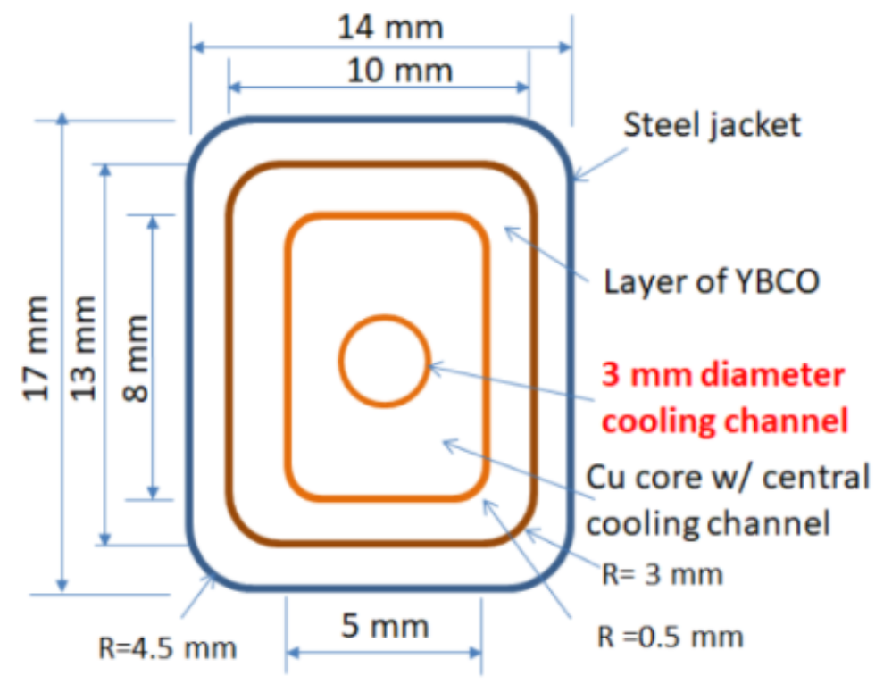
\includegraphics[width =0.5\linewidth]{StandardFigures/yuhu_cs.pdf}
    \caption{HTS cable geometry.}
    \label{fig:yuhu_cs}
\end{figure}

\subsubsection*{22.1.3.3 Shim Coils}

These coils serve to apply fine adjustments to the field profile to maintain field uniformity, and control any plasma disturbances. These cost 275 M USD.\\

\begin{table}[h]
\centering
\resizebox{0.7\linewidth}{!}{%
\begin{tabular}{lccc}
\hline
\textbf{Parameter} & \textbf{Solenoid} & \textbf{Mirror 1} & \textbf{Mirror 2} \\
\hline
Radius (m)& 5.05 & 2.95 & 1.5 \\
dr (m)& 0.779 & 1.46 & 1.46 \\
dz (m)& 0.779 & 1.46 & 1.46 \\
Current supply (kA) & 19.576 & 19.576 & 19.576 \\
Cable current density (A/mm$^2$)& 22.4 & 22.4 & 22.4 \\
Conductor current density (A/mm$^2$) & 150 & 150 & 150 \\
Cable width (m)& 0 & 0 & 0 \\
Cable height (m)& 0 & 0 & 0 \\
Total volume (m$^3$)& 19 & 40 & 20 \\
Cross-sectional area (m$^2$)& 1 & 2 & 2 \\
\hline
Cable turns & 2550 & 8956 & 8956 \\
Turns of conductor/cable & 68 & 68 & 68 \\
Total turns of conductor & 174272 & 612152 & 612152  \\
Length of conductor (km)& 5530 & 11346 & 5769 \\
Current per conductor (A)& 112 & 32 & 32 \\
\hline
Cost of SC (M USD)& 31 & 18 & 9 \\
Cost of copper (M USD)& 0 & 1 & 1 \\
Cost of SS (M USD)& 0 & 0 & 0 \\
Total material cost (M USD)&  32 & 20 & 10 \\
Manufacturing factor (M USD)& 3 & 3 & 3 \\
Structural cost (M USD) & 24 & 15 & 7 \\
Quantity & 9 & 2 & 2 \\
Magnet cost (single)(M USD) & 95 & 59 & 30 \\
Magnet $+$ structure cost (single) (M USD) & 119 & 73 & 37 \\
\hline
Total cost (M USD) & 1071 & 146 & 74 \\
\hline
\end{tabular}
} % end \resizebox
\caption{Design parameters for an individual coil of each of the main coils in this concept. In the concept, there are 2 mirror coils at each end, and 9 equally axially distributed, identical solenoid coils.}
\label{your-table-label}
\end{table}

\subsubsection*{22.1.3.4 Structural cost}

The structural cost for the coils is difficult to cost from first principles without detailed structural analysis with FEM. Here, the approach is a series of analytical estimations of the dominant stresses. These include:

\begin{itemize}
    \item Hoop stress within the coil generated by the cumulative effect of the induced force between concentric radial turns.
    \item Axial force generated between cable turns within the coils. 
    \item Axial force between adjacent coils.
\end{itemize}


By considering these primary contributions, an estimate of the structural material required (such as the hoop restraint requirements) can be calculated. From this preliminary estimate, a structural cost of 25\% of the coil cost is used as a conservative factor. This is in comparison to 50-100\% as the standard for Tokamaks. The structural cost is thus 156704 M USD.


